\documentclass{beamer}

\usepackage{tikz}
\usepackage{tabu}
\usepackage{adjustbox}
\usepackage{graphicx}
\usepackage{tabularx}
\usepackage{multirow}
\usepackage{booktabs}
  \setbeamertemplate{mini frames}{}
  % or ...

\usepackage{hyperref}
\usepackage{pgf,pgfarrows,pgfnodes,pgfpages}
\usepackage[english]{babel}

\usepackage[latin1]{inputenc}

\title[] % (optional, use only with long paper titles)
{\vskip0pt\normalsize{USDA Food Assistance Programs (SNAP, the National School Lunch Program, and the School Breakfast Program) and Healthy Food Choices: Quasi-Experimental Evidence from Geographic Variation in Food Prices}}

\subtitle
{} % (optional)

\author%[Author, Another] % (optional, use only with lots of authors)
{\small{{Erin Todd Bronchetti (Swarthmore College) \\ Garret Christensen (UC Berkeley)\\ Benjamin Hansen (University of Oregon)}}}
% - Use the \inst{?} command only if the authors have different
%   affiliation.

\date[Short Occasion] % (optional)
{November 2017* \\
Preliminary: Please don't cite}


\subject{Talks}
%\titlegraphic{\includegraphics[width=\textwidth,height=.5\textheight]{nudgebanner}}

% This is only inserted into the PDF information catalog. Can be left
% out. 



% If you have a file called "university-logo-filename.xxx", where xxx
% is a graphic format that can be processed by latex or pdflatex,
% resp., then you can add a logo as follows:

% \pgfdeclareimage[height=0.5cm]{university-logo}{university-logo-filename}
% \logo{\pgfuseimage{university-logo}}



% Delete this, if you do not want the table of contents to pop up at
% the beginning of each subsection:
%\AtBeginSubsection[]
%{
%  \begin{frame}<beamer>{Outline}
   % \tableofcontents[currentsection,currentsubsection]
  %\end{frame}
%}


% If you wish to uncover everything in a step-wise fashion, uncomment
% the following command: 

%\beamerdefaultoverlayspecification{<+->}
%\titlegraphic{\includegraphics[width=\textwidth,height=.5\textheight]{someimage}}
%\begin{beameroption}{show only notes{}
\def\tiny{\fontsize{7pt}{7pt}\selectfont}
\setbeamerfont{section in head/foot}{size=\tiny}



\begin{document}

\begin{frame}
  \titlepage
 
  \tiny{\begin{quote}This project was supported with grants from the National Bureau of Economic Research and University of Kentucky Center for Poverty Research through funding by the U.S. Department of Agriculture, Economic Research Service and the Food and Nutrition Service, Agreement Numbers 58-5000-1-0050 and 58-5000-3-0066. The opinions and conclusions expressed herein are solely those of the author(s) and should not be construed as representing the opinions or policies of the sponsoring agencies\end{quote}}
%\note[item]<1>{Thank you all for being here today, during this very busy first week of classes.}
%\note[item]<1>{I, personally, am delighted to be beginning another academic year at Swarthmore...}
%\note[item]<1>{"Portfolio approach" ... projects in several different topic areas ... all connected by an interest in social welfare policy and social insurance...} 
%\note[item]<1>{as well as a focus not just on the COSTS of these programs (incentive effects)... but also on the BENEFITS -- (protect material wellbeing)}
  %\end{singlespacing}
   %\end{reference} 
\end{frame}

%\newcounter{saveenumi}
%\newcommand{\seti}{\setcounter{saveenumi}{\value{enumi}}}
%\newcommand{\conti}{\setcounter{enumi}{\value{saveenumi}}}

%\begin{frame}{Outline}
  %\tableofcontents
  % You might wish to add the option [pausesections]
%\end{frame}

%%%%%%%%%%%%%%%%%%%%%%%%%%%%%%%%%%%%%%%%%%%%%%%%%%%%%%%%%%%%%%%%%%%%%%%%%%%%%%%%%%%%%%
\section{Introduction}

\begin{frame}{SNAP Background}
Food Stamps (i.e. the Supplemental Nutrition Assistance Program, SNAP) is one of the largest government assistance programs.
\begin{itemize}
\item
	More than one in seven Americans
\item
	Cost: \$80 billion FY2013
\item 
	Started in 1964, expanded in 1971, purchase requirement eliminated in 1977
\item 
	Paid for by Feds (the farm bill), administered by states
\item
	Electronic Balance Transfer (EBT) in early 2000s
\end{itemize}
\end{frame}

\begin{frame}{How It Works}
\begin{itemize}
\item Less than \$2,250/\$3,250 in countable assets. (Not home, sometimes car.)
\item Less than net monthly income 100\% of FPL, Gross 130\% (\$2,021/\$2,628 family of 4)
\item Earned income, dependent care, medical expenses, child support, excess shelter deductions.
\item $ Benefits=MaxBenefits(\$649/month)-NetIncome*0.3 $
\end{itemize}
\end{frame}



\begin{frame}{Recent Issues}
\begin{itemize}
\item Massive increase in recipients
\item ARRA: Benefits increased \$80/month in 2009, decreased in 2013.
\item Able bodied without dependents 18-49(ABAWDs) eligibility maxes out at 3/36 months. Waived with high unemployment---kicking back in after Great Recession.
\item Food insecurity among recipient households remains quite high \href{http://www.ers.usda.gov/media/1896841/err194.pdf}{(Coleman-Jensen et al., 2014)}.
\end{itemize}
\end{frame}

\begin{frame}
\begin{figure}
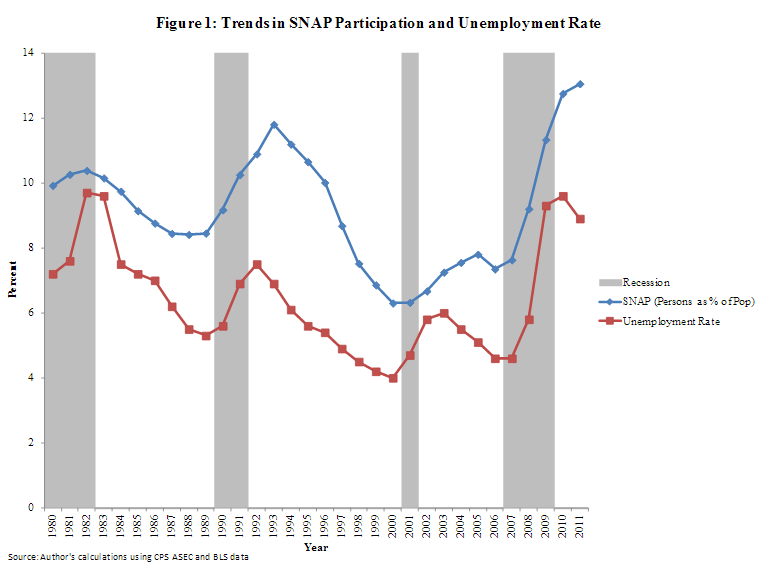
\includegraphics[width=\textwidth]{./images/Ziliak.PNG}

Ziliak 2016
\end{figure}
\end{frame}

\begin{frame}{Our Research I}
\begin{itemize}
\item
 While legislated maximum SNAP benefits are fixed across 48 states, food prices vary significantly across geographic locations.
\item Deductions for costs of housing, medical care, and dependent care help, but are not sufficient sufficient to equalize real value of SNAP benefits across geographic areas \href{http://www.childrenshealthwatch.org/publication/real-cost-of-a-healthy-diet-2011/}{(Breen et al., 2011)}.
\item Food price variation has been studied using BLS data at the census region level, or using \href{http://www.ers.usda.gov/data-products/quarterly-food-at-home-price-database.aspx}{QFAHPD} for 35 market groups \href{http://aepp.oxfordjournals.org/content/35/4/679}{(Gregory \& Coleman-Jensen, 2013)}.
\end{itemize}
\end{frame}

\begin{frame}{Our Research II}
\begin{itemize}
\item
 What fraction of recipients can actually afford the TFP locally?
\item 
\textbf{What does SNAP relative generosity do to nutrition?}
\item Other data: 
 What does SNAP relative generosity do to child health?
\end{itemize}
\end{frame}

%%%%%%%%%%%%%%%%%%%%%%%%%%%%%%%%%%%%%%MAPS%%%%%%%%%%%%%%%%%%%%%%%%%%%%%%%%%%%%%%%%%

{
   \setbeamertemplate{navigation symbols}{}
    \begin{frame}[plain]
        \begin{tikzpicture}[remember picture,overlay]
            \node[at=(current page.center)] {
                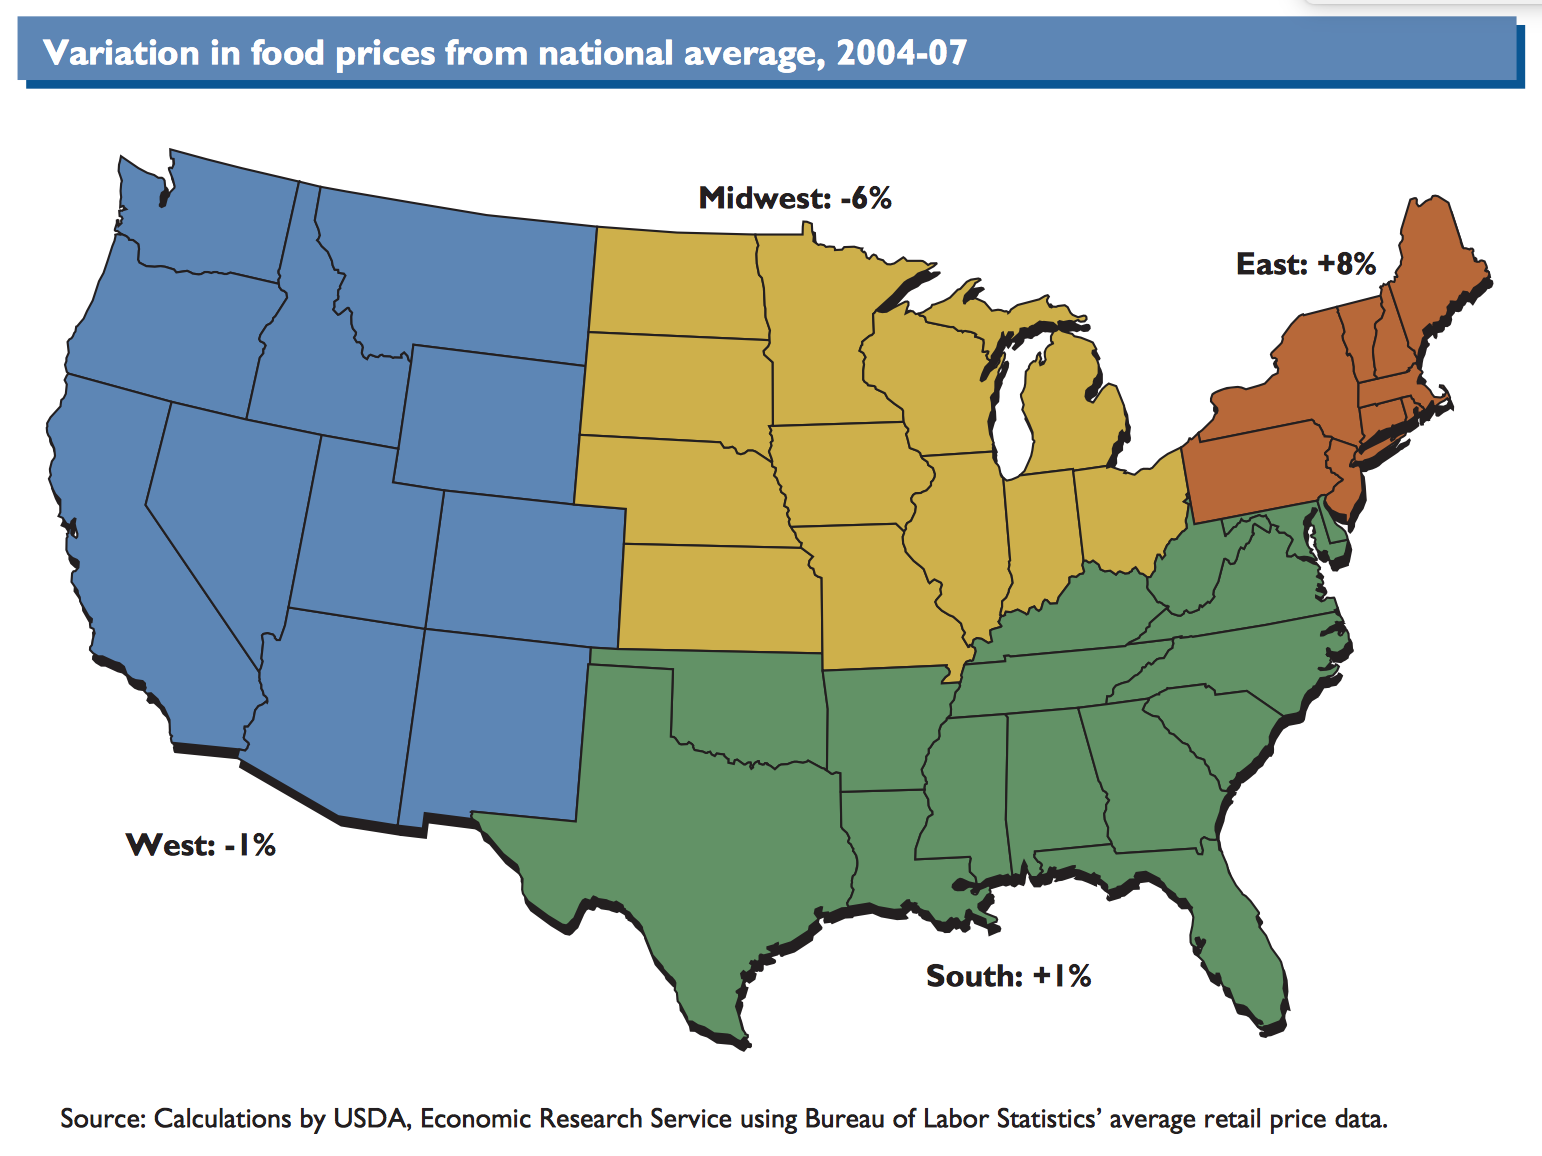
\includegraphics[width=\paperwidth]{./images/region_FPvary_map.png}
            };
        \end{tikzpicture}
     \end{frame}
}

{
   \setbeamertemplate{navigation symbols}{}
    \begin{frame}[plain]
        \begin{tikzpicture}[remember picture,overlay]
            \node[at=(current page.center)] {
                \href{http://www.ers.usda.gov/publications/eib-economic-information-bulletin/eib29-2.aspx}{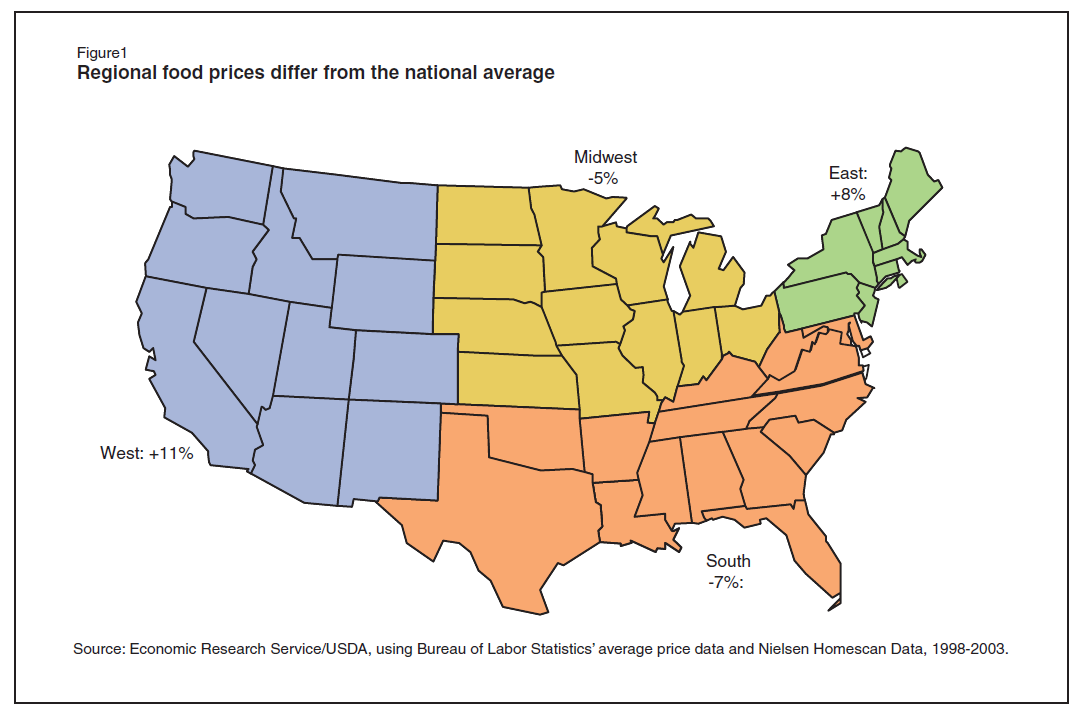
\includegraphics[width=\paperwidth]{./images/region_FPvary_map2.png}}
            };
        \end{tikzpicture}
     \end{frame}
}

{
   \setbeamertemplate{navigation symbols}{}
    \begin{frame}[plain]
        \begin{tikzpicture}[remember picture,overlay]
            \node[at=(current page.center)] {
                \href{http://www.ers.usda.gov/media/176139/page19.pdf}{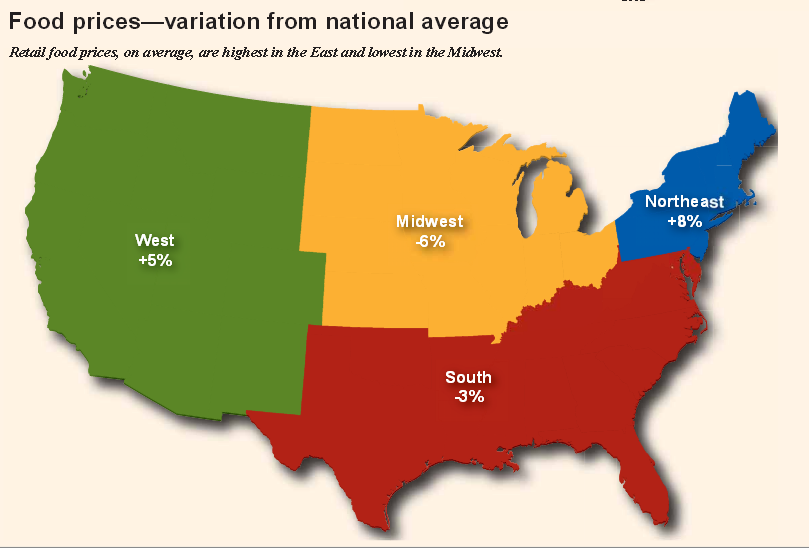
\includegraphics[width=\paperwidth]{./images/region_FPvary_map3.png}}
            };
        \end{tikzpicture}
     \end{frame}
}

%%%%%%%%QFAHPD
{
   \setbeamertemplate{navigation symbols}{}
    \begin{frame}[plain]
        \begin{tikzpicture}[remember picture,overlay]
            \node[at=(current page.center)] {
                \href{http://www.ers.usda.gov/publications/tb-technical-bulletin/tb1926.aspx}{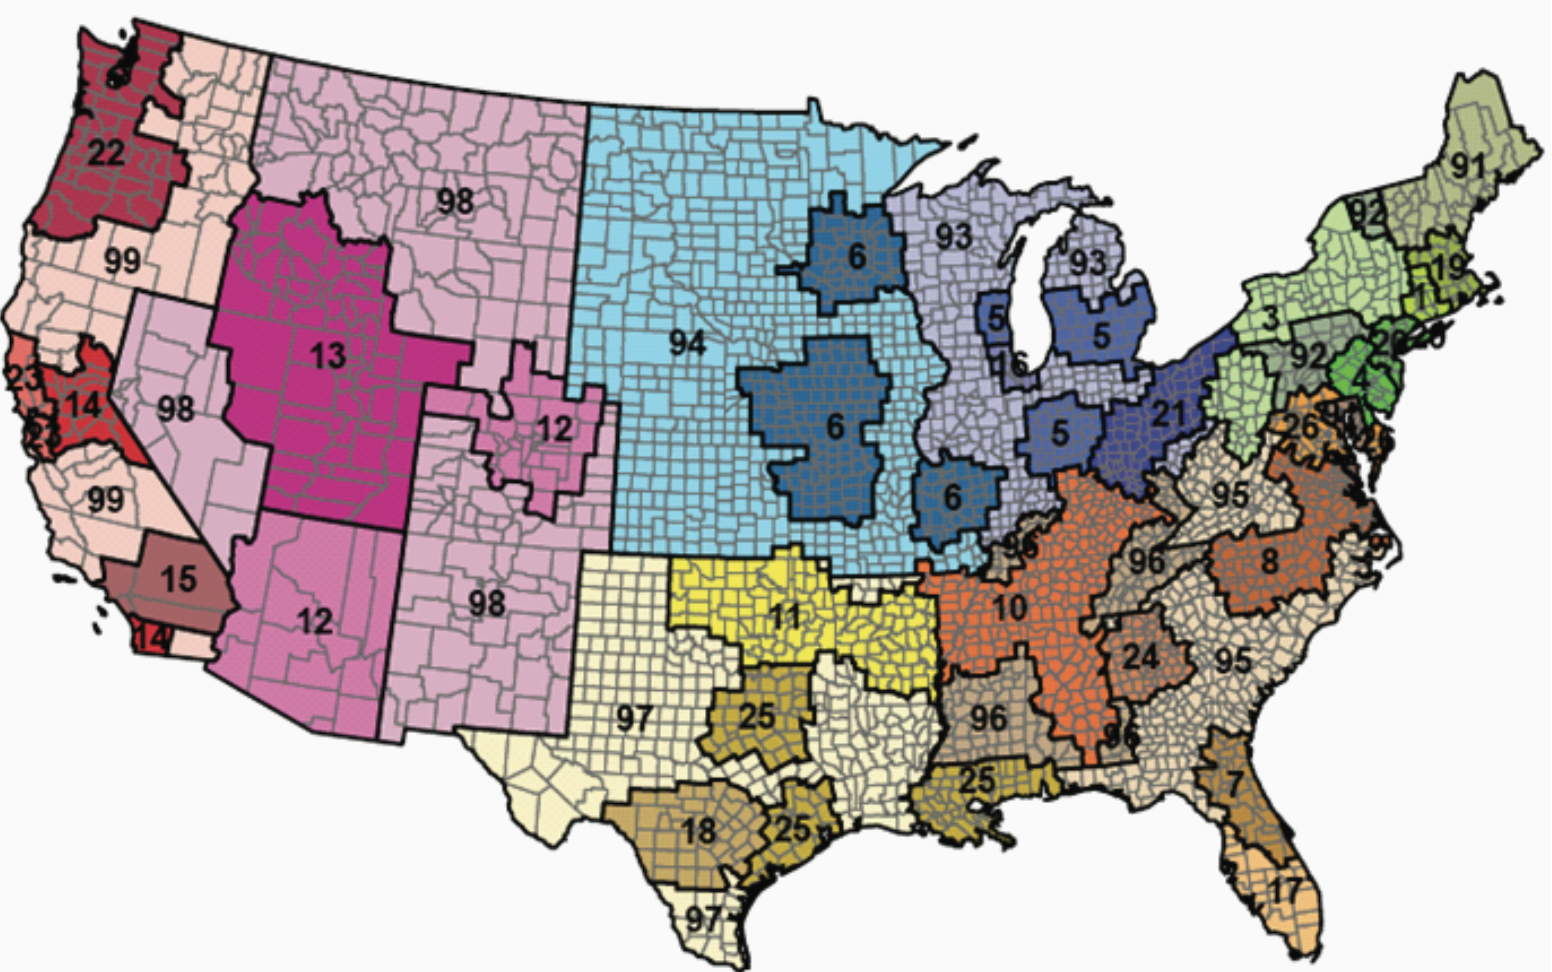
\includegraphics[width=\paperwidth]{./images/mktgrp_FPvary_map}}
            };
        \end{tikzpicture}
     \end{frame}
}

%%%%%OUR RESEARCH%%%%%%%%%%%%

\begin{frame}
Our data: At census block group level, but no map. Sorry!
\end{frame}

{
   \setbeamertemplate{navigation symbols}{}
    \begin{frame}[plain]
        \begin{tikzpicture}[remember picture,overlay]
            \node[at=(current page.center)] {
                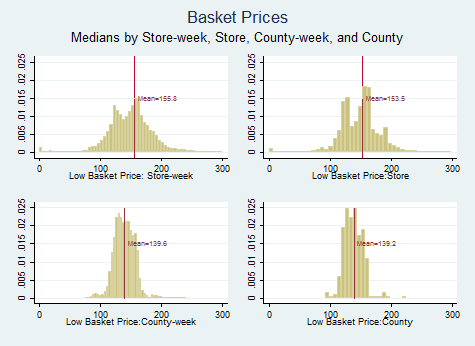
\includegraphics[width=\paperwidth]{./images/ComboBPHisto.png}
            };
        \end{tikzpicture}
     \end{frame}
}

%%%%%%%%%%%%%%%%%%%%%%%%%%%%%%%%%%%%%%%%%%%%%%%%%%%%%%%%%%%%%%%%%%%%%%%%%%%%%%%%%%%%
\begin{frame}{FoodAPS}
``USDA's National Household Food Acquisition and Purchase Survey (FoodAPS) is the first nationally representative survey of American households to collect unique and comprehensive data about household food purchases and acquisitions.''
\begin{itemize}
\item FoodAPS lets us look at the relationship between food prices and SNAP adequacy at a much finer geographical level.
\item  We compare households' SNAP benefits to the prices these households face for a standardized bundle of foods: The Thrifty Food Plan.
\end{itemize}
\end{frame}

\begin{frame}{The Thrifty Food Plan (TFP)}
  \setlength{\leftmargini}{1em}
\begin{itemize}
\item
Well-defined basket of foods to obtain a nutritious diet at a minimal cost.

\item
You're supposed to be able to buy TFP with 30\% of net income + food stamp benefits.

\item That's where the 649 comes from: $ Benefits=MaxBenefits(\$649/month)-NetIncome*0.3 $
\end{itemize}
\end{frame}


\begin{frame}
\begin{figure}
\frame{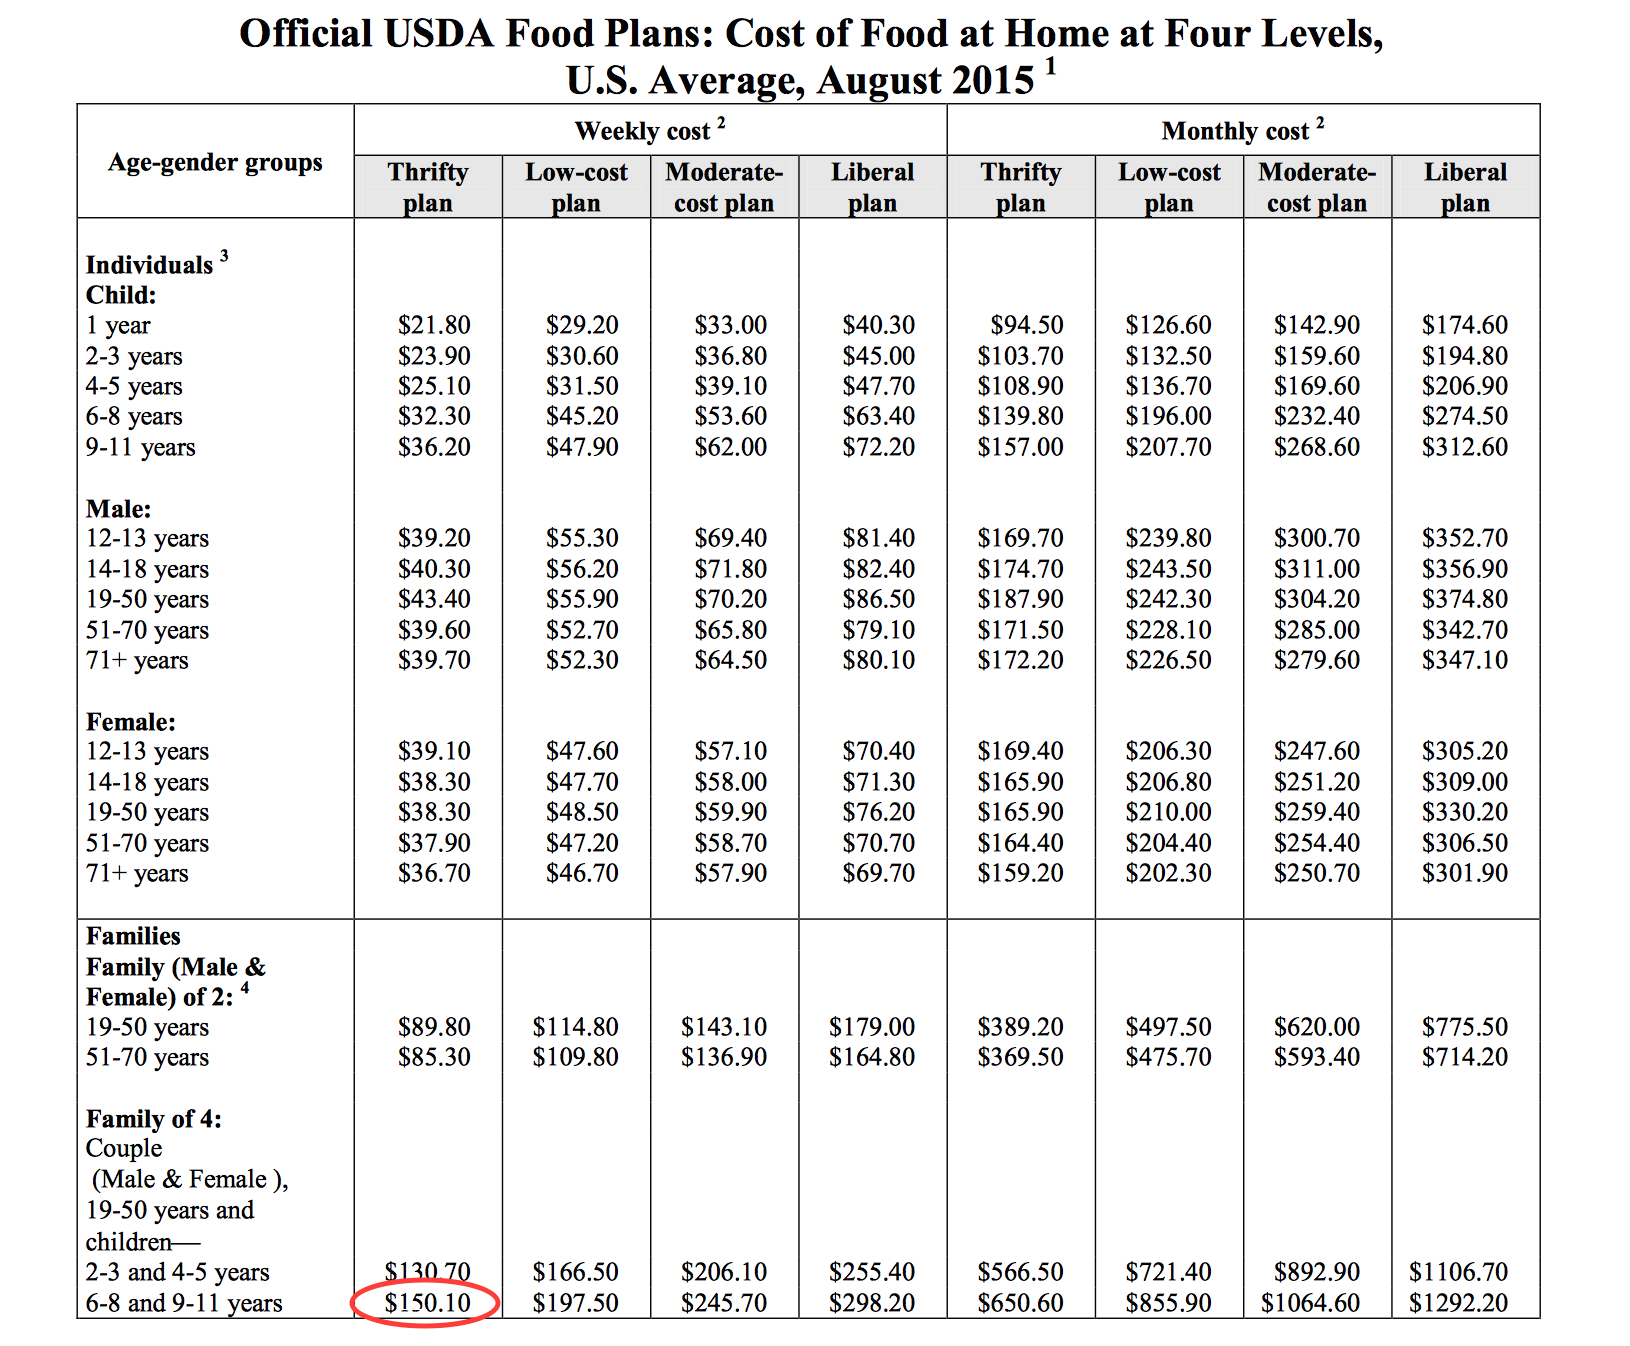
\includegraphics[scale=0.35]{./images/TFPa}}
\end{figure}
\end{frame}
%%%%%%%%%%%%%%%%HISTOGRAMS OF TFP

\begin{frame}
\begin{figure}
{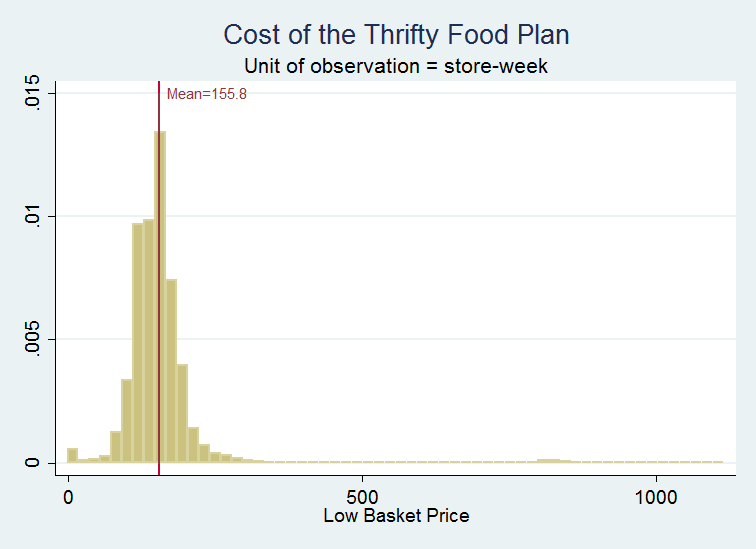
\includegraphics[scale=.4, trim=0cm .0cm 0cm 0cm, clip=true]{./images/low_basket_price_histo.png}}
\end{figure}
\end{frame}
%%%%%%%%%%%%%%%%%%%%%%%%%%%


\begin{frame}{Research Questions}
\begin{enumerate}
\item \large{Are SNAP benefits adequate for SNAP households to purchase the TFP? If not, what is the shortfall?}\\
\vskip6pt \hspace{2mm} \normalsize{\underline{\textit{Compare TFP cost to:}}}
\begin{itemize}
{\item SNAP benefit received + 30\% of gross income} 
{\item SNAP benefit received + 30\% of net income} 
{\item Legislated maximum SNAP benefit} 
\end{itemize}
{\item \vskip12pt \large{What about for SNAP-eligible households?}}\\
{\item \vskip12pt \large{For which types of households are SNAP benefits inadequate?}}
\end{enumerate}
\end{frame}

%%%%%%%%%%%%%%%%%%%%%%%%%%%%%%%%%%%%%%%%%%%%%%%%%%%%%%%%%%%%%%%%%%%%%%%%%%%%%%%%%%%
\begin{frame}

% Table generated by Excel2LaTeX from sheet 'Tcounty-st-cr-suff'
\begin{table}[htbp]{Sufficiency Rates of SNAP for \textbf{Recipient} Households by Distance from Stores}

\begin{adjustbox}{height=1.5in}
  \centering
    \begin{tabular}{lllllll}
    \toprule
          & Average & Standard Error & N     & Average & Standard Error & N \\

     & \multicolumn{3}{c}{Net Income} & \multicolumn{3}{c}{Max Benefits} \\

    \midrule
    Census Region Median & 78\%  & 0.02  & 1444  & 83\%  & 0.03  & 1581 \\
    State Median & 79\%  & 0.02  & 1444  & 76\%  & 0.04  & 1581 \\
    County Median & 79\%  & 0.02  & 1436  & 74\%  & 0.04  & 1572 \\
    20-mile Median & 78\%  & 0.02  & 1338  & 73\%  & 0.04  & 1464 \\
    10-mile Median & 78\%  & 0.02  & 1311  & 73\%  & 0.04  & 1433 \\
    5-mile Median & 77\%  & 0.02  & 1224  & 72\%  & 0.04  & 1338 \\
    3.4-mile Median & 77\%  & 0.02  & 1174  & 74\%  & 0.04  & 1281 \\
    2.5mile Median & 77\%  & 0.02  & 1123  & 72\%  & 0.04  & 1225 \\
    10-nearest Median & 79\%  & 0.02  & 1338  & 77\%  & 0.03  & 1464 \\
    5-nearest Median & 78\%  & 0.02  & 1332  & 71\%  & 0.03  & 1458 \\
          &       &       &       &       &       &  \\

    Census Region Minimum & 100\% & 0.00  & 1444  & 100\% & 0.00  & 1581 \\
    State Minimum & 99\%  & 0.00  & 1444  & 100\% & 0.00  & 1581 \\
    County Minimum & 94\%  & 0.01  & 1436  & 100\% & 0.00  & 1572 \\
    20-mile Minimum & 95\%  & 0.01  & 1338  & 100\% & 0.00  & 1464 \\
    10-mile Minimum & 93\%  & 0.01  & 1311  & 100\% & 0.00  & 1433 \\
    5-mile Minimum & 91\%  & 0.01  & 1224  & 99\%  & 0.00  & 1338 \\
    3.4-mile Minimum & 90\%  & 0.01  & 1174  & 100\% & 0.00  & 1281 \\
    2.5mile Minimum & 90\%  & 0.01  & 1123  & 99\%  & 0.01  & 1225 \\
    10-nearest Minimum & 91\%  & 0.01  & 1338  & 100\% & 0.00  & 1464 \\
    5-nearest Minimum & 89\%  & 0.01  & 1332  & 98\%  & 0.01  & 1458 \\
    2-nearest Minimum & 83\%  & 0.02  & 1332  & 85\%  & 0.02  & 1458 \\
    \bottomrule
    \end{tabular}
    \end{adjustbox}
	\end{table}

\end{frame}


%%%%%%%%%%%%%%%%%%%%%%%%%%%%%%%%%%%%%%%%%%%%%%%%%%%%%%%%%%%%%%%%%%%%%%%%%%%%
%%%%%%%%%%%%%%%%%%%%%%%%%%%%%%%%%%%%%%%%%%%%%%%%%%%%%%%%%%%%%%%%%%%%%%%%%
%\begin{frame}
%\begin{figure}
%{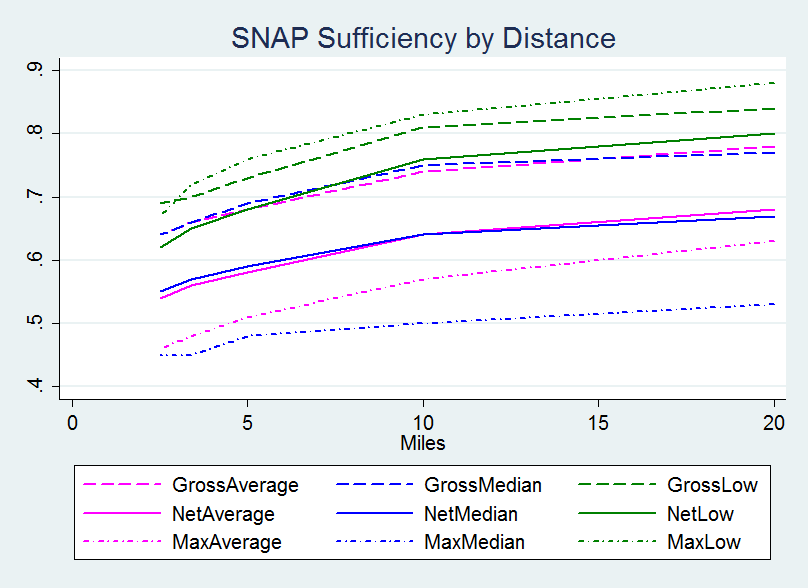
\includegraphics[scale=.4, trim=0cm .0cm 0cm 0cm, clip=true]{./images/quicklinegraph.png}}
%\end{figure}
%\end{frame}

%%%%%%%%%%%%%%%%%%%%%%%%%%%%%%%%%%%%%%%%%%%%%%%%%%%%%%%%%%%%%%%%%%%%%%%%
% Table generated by Excel2LaTeX from sheet 'Tdist-suffEL'
\begin{frame}
\begin{table}[htbp]{Sufficiency Rates of SNAP for \textbf{Eligible} Households by Distance from Stores}

\begin{adjustbox}{height=1.5in}
    
    \begin{tabular}{lllllll}
    \toprule
          & Average & Standard Error & N     & Average & Standard Error & N \\
    \midrule
     & \multicolumn{3}{c}{Simulated Benefits} & \multicolumn{3}{c}{Max Benefits} \\
    
    Region Median & 94\%  & 0.01  & 2405  & 78\%  & 0.03  & 2405 \\
    State Median & 93\%  & 0.01  & 2405  & 73\%  & 0.03  & 2405 \\
    County Median & 93\%  & 0.01  & 2395  & 71\%  & 0.05  & 2395 \\
    20-mile Median & 92\%  & 0.01  & 2242  & 69\%  & 0.05  & 2242 \\
    10-mile Median & 92\%  & 0.01  & 2189  & 68\%  & 0.04  & 2189 \\
    5-mile Median & 91\%  & 0.01  & 2043  & 67\%  & 0.04  & 2043 \\
    3.4-mile Median & 91\%  & 0.01  & 1962  & 68\%  & 0.04  & 1962 \\
    2.5mile Median & 92\%  & 0.01  & 1879  & 68\%  & 0.04  & 1879 \\
    10-nearest Median & 93\%  & 0.01  & 2242  & 72\%  & 0.03  & 2242 \\
    5-nearest Median & 92\%  & 0.01  & 2237  & 64\%  & 0.03  & 2237 \\
          &       &       &       &       &       &  \\
    Region Minimum & 100\% & 0.00  & 2405  & 100\% & 0.00  & 2405 \\
    State Minimum & 100\% & 0.00  & 2405  & 100\% & 0.00  & 2405 \\
    County Minimum & 100\% & 0.00  & 2395  & 100\% & 0.00  & 2395 \\
    20-mile Minimum & 100\% & 0.00  & 2242  & 99\%  & 0.01  & 2242 \\
    10-mile Minimum & 100\% & 0.00  & 2189  & 100\% & 0.00  & 2189 \\
    5-mile Minimum & 99\%  & 0.00  & 2043  & 98\%  & 0.00  & 2043 \\
    3.4-mile Minimum & 99\%  & 0.00  & 1962  & 98\%  & 0.01  & 1962 \\
    2.5mile Minimum & 99\%  & 0.00  & 1879  & 97\%  & 0.01  & 1879 \\
    10-nearest Minimum & 100\% & 0.00  & 2242  & 99\%  & 0.01  & 2242 \\
    5-nearest Minimum & 99\%  & 0.00  & 2237  & 97\%  & 0.01  & 2237 \\
    2-nearest Minimum & 96\%  & 0.00  & 2237  & 82\%  & 0.02  & 2237 \\
    \bottomrule
\end{tabular}
\end{adjustbox}
\end{table}
\end{frame}

%%%%%%%%%%%%%%%%%%%%%%%%%%%%%%%%%%%%%%%%%%%%%%%%%%%%%%%%%%%%%%%%%%%%%%%
% Table generated by Excel2LaTeX from sheet 'Tdist-gap'
%\begin{frame}
%\begin{table}[htbp]{Dollar Gap between SNAP and TFP for Recipient Households by Distance from Store}
%\begin{adjustbox}{max width=\textwidth}
%  \centering
%    \begin{tabular}{llllllllll}
%    \toprule
%    \midrule
%          & \multicolumn{3}{l}{Gross Income} & \multicolumn{3}{l}{Net Income} & \multicolumn{3}{l}{Max Benefits} \\
%    TFP Calculation & Mean & S.E. & N     & Mean & S.E. & N     & Mean & S.E. & N \\
%    Primary Store & 122.35 & --    & 86    & 118.07 & --    & 173   & 41.19 & --    & 255 \\
%    Alternate Store & 150.53 & --    & 54    & 154.66 & --    & 106   & 49.33 & --    & 157 \\
%    Primary and Alt Mean & 145.72 & --    & 105   & 127.14 & --    & 224   & 41.84 & --    & 282 \\
%    20-mile Mean & 137.69 & --    & 171   & 153.89 & --    & 327   & 35.19 & --    & 422 \\
%    20-mile Median & 121.04 & --    & 167   & 141.40 & --    & 335   & 22.25 & --    & 509 \\
%    20-mile Minimum & 77.03 & --    & 48    & 99.21 & --    & 104   & 15.87 & --    & 2 \\
%    10-mile Mean & 141.62 & --    & 170   & 151.67 & --    & 324   & 39.77 & --    & 433 \\
%    10-mile Median & 133.20 & --    & 161   & 144.44 & --    & 313   & 24.10 & --    & 498 \\
%    10-mile Minimum & 97.35 & --    & 59    & 108.68 & --    & 124   & 30.11 & --    & 14 \\
%    5-mile Mean & 142.27 & --    & 162   & 151.16 & --    & 315   & 38.47 & --    & 426 \\
%    5-mile Median & 135.35 & --    & 158   & 150.97 & --    & 300   & 28.81 & --    & 462 \\
%    5-mile Minimum & 106.25 & --    & 68    & 117.23 & --    & 148   & 21.33 & --    & 34 \\
%    3.4-mile Mean & 147.17 & --    & 161   & 156.81 & --    & 306   & 41.57 & --    & 420 \\
%    3.4-mile Median & 125.05 & --    & 160   & 147.47 & --    & 294   & 28.99 & --    & 454 \\
%    3.4-mile Minimum & 105.63 & --    & 77    & 119.16 & --    & 163   & 22.38 & --    & 51 \\
%    2.5-mile Mean & 139.27 & --    & 160   & 149.41 & --    & 295   & 47.19 & --    & 420 \\
%    2.5-mile Median & 130.23 & --    & 150   & 146.21 & --    & 287   & 34.81 & --    & 447 \\
%    2.5-mile Minimum & 108.30 & --    & 79    & 121.42 & --    & 170   & 25.57 & --    & 92 \\
%    \bottomrule
%\end{tabular}
%\end{adjustbox}
%\end{table}
%\end{frame}


%%%%%%%%%%%%%%%%%%%%%%%%%%%%%%%%%%%%%%%%%%%%%%%%%%%%%%%%%%%%%%%%%%%%%%%%%%%%%%%%%%%%%%%%%%
\begin{frame}
% Table generated by Excel2LaTeX from sheet 'Tcharacteristics'
\begin{table}{Characteristics of Households by SNAP Sufficiency}%[htbp]

\begin{adjustbox}{max width=\textwidth}
  \centering
  %\caption{}
     \begin{tabular}{lllllll}
    \toprule
    & \multicolumn{3}{l}{SNAP Recipients} & \multicolumn{3}{l}{SNAP Eligible} \\

    Characteristic & No    & Yes   & P-value & No    & Yes   & P-value \\
    \midrule
    Family Size & 2.78  & 2.65  & 0.43  & 2.52  & 2.21  & 0.11 \\
    Household Max Age & 50.83 & 49.35 & 0.30  & 53.22 & 53.00 & 0.89 \\
    Household Min Age & 27.00 & 28.14 & 0.65  & 34.82 & 37.21 & 0.43 \\
    Income Per Person & 952.04 & 894.23 & 0.52  & 1571.35 & 1354.35 & 0.18 \\
    Income & 2392.80 & 1950.32 & 0.05  & 3059.18 & 2355.08 & 0.04 \\
    Percent of Poverty Line & 141.95 & 124.20 & 0.12  & 209.82 & 172.74 & 0.08 \\
    HH Has Earned Income & 0.50  & 0.53  & 0.57  & 0.60  & 0.55  & 0.21 \\
    Household Max Education & 20.08 & 19.65 & 0.10  & 20.76 & 20.24 & 0.09 \\
    HH Has Elderly Member & 0.30  & 0.27  & 0.40  & 0.38  & 0.37  & 0.83 \\
    Nonmetro Area & 0.03  & 0.17  & 0.01  & 0.03  & 0.17  & 0.02 \\
    Metro Area & 0.97  & 0.83  & 0.01  & 0.97  & 0.83  & 0.02 \\
    High Food Security & 0.34  & 0.32  & 0.52  & 0.45  & 0.50  & 0.44 \\
    Marginal Food Security & 0.25  & 0.21  & 0.24  & 0.23  & 0.19  & 0.13 \\
    Low Food Security & 0.24  & 0.26  & 0.57  & 0.21  & 0.16  & 0.08 \\
    Very Low Food Security & 0.18  & 0.21  & 0.40  & 0.11  & 0.16  & 0.02 \\
    Troube Paying Bills & 0.30  & 0.27  & 0.45  & 0.18  & 0.17  & 0.83 \\
    High Price Area & 0.88  & 0.00  & 0.00  & 0.90  & 0.00  & 0.00 \\
    Northeast & 0.22  & 0.09  & 0.25  & 0.29  & 0.09  & 0.13 \\
    Midwest & 0.24  & 0.34  & 0.33  & 0.16  & 0.35  & 0.05 \\
    South & 0.33  & 0.43  & 0.25  & 0.32  & 0.42  & 0.33 \\
    West  & 0.21  & 0.14  & 0.49  & 0.22  & 0.14  & 0.39 \\

    
    \bottomrule
\end{tabular}
\end{adjustbox}
\end{table}
\end{frame}


%%%%%%%%%%%%%%%%%%%%%%%%%%%%%%%%%%%%%%%%%%%%%%%%%%%%%%%%%%%%%%%%%%%%%%%%%%%%%%%%%%%%%%%%
\section{Conclusions}

\begin{frame}{Conclusions and Concerns from Variation in Sufficiency}
 
Bronchetti, Christensen, Hansen
 
\begin{enumerate}
\item 
Fraction of SNAP households who can afford to purchase the TFP within their county 75\% to 80\%.

\begin{itemize}
\item Matters less what shopping radius you use than whether people can find and shop at minimum store.

\end{itemize}
\item 
Estimated measures of SNAP adequacy are higher among SNAP-eligible households than SNAP recipients, with results dependent on benefit calculation method.
\item 
Families in high-price and perhaps metro areas are less able to afford the TFP.

\item Gap measure hard to define in useful relative terms (zero/very low income, benefits).
\end{enumerate}
\end{frame}

%%%%%%%%%%%%%%%%%%%%%%%%%%%%%%%%%%%%%%%%%%%%
\begin{frame}{Health Effects}
 Bronchetti, Christensen, Hoynes
 
\href{http://www.ukcpr.org/sites/www.ukcpr.org/files/UKCPR\%20Grant\%20Winners\%20Announcement.pdf}{The Real Value of SNAP Benefits and Health Outcomes}
\begin{itemize}
\item Use QFAHPD and restricted access geo-located NHIS to look at how food price variation affects health outcomes among SNAP recipients and SNAP eligibles (UKCPR).
\item 
10 percent increase in SNAP purchasing power increases the likelihood a child had a check-up in the past year by 5.4 percent and may reduce the likelihood that children delay or go without care due to cost.
\item
We do not find much evidence that these higher prices cause detrimental impacts on health status, the likelihood of a hospitalization, or other measures of physical (e.g., obesity) and mental health (e.g., child has emotional problems). School days is exception.
\end{itemize}
\end{frame}

\begin{frame}
\begin{table}{Health Care Utilization}%[htbp]

\begin{adjustbox}{max width=\textwidth}
  \centering
      \begin{tabular}{lccc}
    
       \toprule
          & (1)   & (2)   & (3) \\
    \midrule
          & Had a & Doctor's & Delay or \\
          & checkup & visit & forgo care \\
          & past 12m & past 12m & past 12m \\
          &       &       &  \\
    log(SNAPMAX/TFP) & 0.435** & 0.221 & -0.148** \\
          & (0.205) & (0.141) & (0.068) \\
          &       &       &  \\
    Mean of dep. var. & 0.766 & 0.895 & 0.0563 \\
    Effect of 10\% increase in SNAP purchasing power & 0.041 & 0.021 & -0.014 \\
    As a \% of mean of dep. var. & \textbf{5.4\%} & 2.3\% & \textbf{-24.9\%} \\
    N     & 18,746 & 18,884 & 18,884 \\
    R2    & 0.083 & 0.043 & 0.020 \\
    \bottomrule
\end{tabular}
\end{adjustbox}
\end{table}
\end{frame}


\begin{frame}
\begin{table}{Health Outcomes}%[htbp]

\begin{adjustbox}{max width=\textwidth}
  \centering
      \begin{tabular}{lccc}
    \toprule
          & (1)   & (2)   & (3) \\
    \midrule
          & Health status & Hospitalized & School days \\
          & excellent or & overnight & missed due \\
          & very good & past 12m & to illness \\
          &       &       &  \\
    log(SNAPMAX/TFP) & -0.106 & 0.080 & -10.340** \\
          & (0.185) & (0.079) & (3.873) \\
          &       &       &  \\
    Mean of dep. var. & 0.701 & 0.078 & 4.956 \\
    Effect of 10\% increase in SNAP purchasing power & -0.010 & 0.000 & -0.986 \\
    As a \% of mean of dep. var. & -1.4\% & 0.0\% & \textbf{-19.9\%} \\
    N     & 18,880 & 18,872 & 11,942 \\
    R2    & 0.034 & 0.150 & 0.038 \\
    \bottomrule
\end{tabular}
\end{adjustbox}
\end{table}
\end{frame}

%%%%%%%%%%%%%%%%%%%%%%%%%%%%%%%%%%%%%%%%%%%%%%%%
\begin{frame}{Nutrition}
 Bronchetti, Christensen, Hansen
\begin{itemize}
\item Use local relative generosity of SNAP to measure nutrition impacts.
\item Outcomes: 
\begin{itemize}
\item HEI (total, fruit, veg)
\item sugar, fat, alcohol (sofa\_perc)
\item self-reported nutrition status
\end{itemize}
\item Cross-sectional data: use Altonji, Elder, Taber method to compare with and without observable controls.
\item National School Lunch Program and the School Breakfast Program as mediators.
\end{itemize}

\end{frame}


%%%%%%%%%%%%%%%%%%%%%%%%%%%%%%%%%%%%%%%%%%%
\begin{frame}{Nutrition}
 $$Nutrition_{ij}=\alpha + \beta \cdot f(TFP_{ij}, MAXSNAP_{ij}) + X_{ij} \cdot \theta + \delta_{j}+\epsilon_{ij} $$
 
\begin{itemize}
\item Function could be $log (TFP_{ij})$, $log(SNAPMAX_{ij}/TFP_{ij})$, sufficiency[0/1], or gap[cont.].
\item $X$ is rural, nonmetro, troublebills, largeexp, highpricearea, inchhavg, famsize, nocar, anytobacco, snapdays\_final, WIC eligibility.
\item County fixed effects for now.
\end{itemize}
\end{frame}


\begin{frame}{Nutrition}
Table I: SNAP purchasing power
\end{frame}

\begin{frame}{Nutrition}
Table II: Binary measure of sufficiency
\end{frame}

\begin{frame}{Nutrition}
Table III: Measure shortfall/surplus
\end{frame}

\begin{frame}{Nutrition}
Very tentative conclusions
 
\begin{itemize}
\item Higher real value of SNAP associated with higher HEI score, evenly across sub-categories.
\item Drop in sugar, fat, and alcohol.
\item Less strong when filtered through exact TFP cost.
\end{itemize}
\end{frame}
%%%%%%%%%%%%%%%%%%%%%%%%%%%%%%%%%%%%%%%%%%%%%%%%%%%%%
\begin{frame}[plain]
\hspace{34mm}
\color{blue!60!black!60}{\Huge{Thank You}}
\end{frame}

\end{document}
